\documentclass[12pt,a4paper]{exam}

\usepackage{iftex}
\ifPDFTeX
  \usepackage{cmap}
  \usepackage[utf8]{inputenc}
  \usepackage[T1]{fontenc}
  \usepackage[english]{babel}
  \usepackage{lmodern}
\else
  \usepackage{fontspec}
  \usepackage[english]{babel}
  \defaultfontfeatures{Ligatures=TeX}
  \setmainfont{Latin Modern Roman}
\fi

\newlength{\TopPageMargin}
\setlength{\TopPageMargin}{0.2cm}
\usepackage[a4paper,left=1cm,right=1cm,top=\TopPageMargin,bottom=1cm]{geometry}
\usepackage{amsmath}
\usepackage{array}
\usepackage{booktabs}
\usepackage{graphicx}
\usepackage{enumitem}
\usepackage{multirow}
\usepackage{ragged2e}
\usepackage{tikz}
\usepackage{eso-pic}
\usepackage{lipsum}
\usepackage{xcolor}
%\printanswers
\unframedsolutions
\pagestyle{empty}
\setlength{\parindent}{0pt}
\renewcommand{\questionlabel}{\textbf{\thequestion)}}
\renewcommand{\questionshook}{%
  \settowidth{\leftmargin}{\textbf{10)}\hskip\labelsep}%
  \labelwidth\leftmargin
  \advance\labelwidth-\labelsep
}
\renewcommand{\solutiontitle}{\noindent\textbf{Answer:}\enspace}

% Measurements are kept in one place to use the same top template on all pages.
\newlength{\TopTableWidth}
\setlength{\TopTableWidth}{\dimexpr\paperwidth-2cm\relax}
\newlength{\TopTableLeft}
\setlength{\TopTableLeft}{1cm}
\newlength{\TopTableTop}
\setlength{\TopTableTop}{\TopPageMargin}
\newlength{\FirstTableHeight}
\setlength{\FirstTableHeight}{3.4cm}
\newlength{\LeftColWidth}
\setlength{\LeftColWidth}{0.26\TopTableWidth}
\newlength{\MidColWidth}
\setlength{\MidColWidth}{0.50\TopTableWidth}
\newlength{\RightColWidth}
\setlength{\RightColWidth}{\dimexpr\TopTableWidth-\LeftColWidth-\MidColWidth\relax}
\newlength{\BetweenTablesGap}
\setlength{\BetweenTablesGap}{1cm}
\newlength{\HeaderToStudentGap}
\setlength{\HeaderToStudentGap}{-0.6cm}
\newlength{\TopRowHeight}
\setlength{\TopRowHeight}{0.9cm}
\newlength{\BotRowHeight}
\setlength{\BotRowHeight}{2.2cm}
\newlength{\StudentTableGap}
\setlength{\StudentTableGap}{0.12cm}
\newlength{\StudentToScoreGap}
\setlength{\StudentToScoreGap}{0.45cm}
\newlength{\StudentHeaderHeight}
\setlength{\StudentHeaderHeight}{0.8cm}
\newlength{\StudentBodyHeight}
\setlength{\StudentBodyHeight}{1.2cm}
\newlength{\StudentLeftColWidth}
\setlength{\StudentLeftColWidth}{0.24\TopTableWidth}
\newlength{\StudentMidColWidth}
\setlength{\StudentMidColWidth}{0.52\TopTableWidth}
\newlength{\StudentRightColWidth}
\setlength{\StudentRightColWidth}{\dimexpr\TopTableWidth-\StudentLeftColWidth-\StudentMidColWidth\relax}
\newlength{\ScoreToProgramGap}
\setlength{\ScoreToProgramGap}{0.18cm}
\newlength{\ProgramHeaderHeight}
\setlength{\ProgramHeaderHeight}{0.65cm}
\newlength{\ProgramRowHeight}
\setlength{\ProgramRowHeight}{0.58cm}
\newlength{\ContentTopOffset}
\setlength{\ContentTopOffset}{\dimexpr
  \TopTableTop+\FirstTableHeight+\HeaderToStudentGap+\StudentHeaderHeight+\StudentBodyHeight+
  \StudentToScoreGap+\TopRowHeight+\BotRowHeight+\ScoreToProgramGap+
  \ProgramHeaderHeight+5\ProgramRowHeight+0.6cm\relax}

% Top margin for question pages (only general info + student table)
\newlength{\QuestionTopOffset}
\setlength{\QuestionTopOffset}{\dimexpr
  \TopTableTop+\FirstTableHeight+\HeaderToStudentGap+\StudentHeaderHeight+\StudentBodyHeight-0.9cm\relax}

\newcommand{\DrawPageTemplate}{%
  \begin{tikzpicture}[remember picture,overlay]
    \begin{scope}[shift={(current page.north west)}]
    % 1 row 3 column table
    \draw[line width=0.4pt,draw=white]
      (\TopTableLeft,-\TopTableTop) rectangle ++(\TopTableWidth,-\FirstTableHeight);
    \draw[line width=0.4pt,draw=white]
      (\TopTableLeft+\LeftColWidth,-\TopTableTop) --
      ++(0,-\FirstTableHeight);
    \draw[line width=0.4pt,draw=white]
      (\TopTableLeft+\LeftColWidth+\MidColWidth,-\TopTableTop) --
      ++(0,-\FirstTableHeight);

    \node[anchor=center] at
      (\TopTableLeft+0.5\LeftColWidth,-\dimexpr\TopTableTop+0.5\FirstTableHeight\relax)
      {
\includegraphics[width=0.99\LeftColWidth,height=2.4cm,keepaspectratio]{logos/logoan.png}};

    \node[anchor=north west,text width=\dimexpr\MidColWidth-0.5cm\relax] at
      (\TopTableLeft+\LeftColWidth+0.25cm,-\TopTableTop-0.25cm)
      {\small\RaggedRight
      Faculty: Engineering\par
      Department: \dotfill\par
      Course Code/Name: MAT 204 Probability and Statistics for Engineers\par
      Instructor: \dotfill};

    \node[anchor=north west,text width=\dimexpr\RightColWidth-0.5cm\relax] at
      (\TopTableLeft+\LeftColWidth+\MidColWidth+0.25cm,-\TopTableTop-0.25cm)
      {\small\RaggedRight
      \textbf{Exam Document}\par
      \textbf{MIDTERM EXAM}\par\vspace{0.15cm}
      Date: 29/03/2026\par
      Duration: 75 minutes};

    % Student information table
    \draw[line width=0.5pt]
      (\TopTableLeft,-\dimexpr\TopTableTop+\FirstTableHeight+\HeaderToStudentGap\relax)
      rectangle ++(\TopTableWidth,-\dimexpr\StudentHeaderHeight+\StudentBodyHeight\relax);
    \draw[line width=0.5pt]
      (\TopTableLeft+\StudentLeftColWidth,-\dimexpr\TopTableTop+\FirstTableHeight+\HeaderToStudentGap\relax)
      -- ++(0,-\dimexpr\StudentHeaderHeight+\StudentBodyHeight\relax);
    \draw[line width=0.5pt]
      (\TopTableLeft+\StudentLeftColWidth+\StudentMidColWidth,-\dimexpr\TopTableTop+\FirstTableHeight+\HeaderToStudentGap\relax)
      -- ++(0,-\dimexpr\StudentHeaderHeight+\StudentBodyHeight\relax);
    \draw[line width=0.5pt]
      (\TopTableLeft,-\dimexpr\TopTableTop+\FirstTableHeight+\HeaderToStudentGap+\StudentHeaderHeight\relax)
      -- ++(\TopTableWidth,0);

    \node[anchor=center] at
      (\TopTableLeft+0.5\StudentLeftColWidth,
      -\dimexpr\TopTableTop+\FirstTableHeight+\HeaderToStudentGap+0.5\StudentHeaderHeight\relax)
      {\small\textbf{Student ID}};
    \node[anchor=center] at
      (\TopTableLeft+\StudentLeftColWidth+0.5\StudentMidColWidth,
      -\dimexpr\TopTableTop+\FirstTableHeight+\HeaderToStudentGap+0.5\StudentHeaderHeight\relax)
      {\small\textbf{Student Name-Surname}};
    \node[anchor=center] at
      (\TopTableLeft+\StudentLeftColWidth+\StudentMidColWidth+0.5\StudentRightColWidth,
      -\dimexpr\TopTableTop+\FirstTableHeight+\HeaderToStudentGap+0.5\StudentHeaderHeight\relax)
      {\small\textbf{Signature}};

    % Questions/scores table
    \draw[line width=0.5pt]
      (\TopTableLeft,-\dimexpr\TopTableTop+\FirstTableHeight+\HeaderToStudentGap+\StudentHeaderHeight+\StudentBodyHeight+\StudentToScoreGap\relax)
      rectangle ++(\TopTableWidth,-\dimexpr\TopRowHeight+\BotRowHeight\relax);
    \draw[line width=0.5pt]
      (\TopTableLeft,-\dimexpr\TopTableTop+\FirstTableHeight+\HeaderToStudentGap+\StudentHeaderHeight+\StudentBodyHeight+\StudentToScoreGap+\TopRowHeight\relax)
      -- ++(\TopTableWidth,0);
    \foreach \i in {1,...,6} {
      \draw[line width=0.5pt]
        (\TopTableLeft+\i*\TopTableWidth/7,-\dimexpr\TopTableTop+\FirstTableHeight+\HeaderToStudentGap+\StudentHeaderHeight+\StudentBodyHeight+\StudentToScoreGap\relax)
        -- ++(0,-\dimexpr\TopRowHeight+\BotRowHeight\relax);
    }

        
    \node[anchor=center] at
      (\TopTableLeft+0.5*\TopTableWidth/7,
      -\dimexpr\TopTableTop+\FirstTableHeight+\HeaderToStudentGap+\StudentHeaderHeight+\StudentBodyHeight+\StudentToScoreGap+0.5\TopRowHeight\relax)
      {\small\textbf{Questions}};
    \node[anchor=center] at
      (\TopTableLeft+1.5*\TopTableWidth/7,
      -\dimexpr\TopTableTop+\FirstTableHeight+\HeaderToStudentGap+\StudentHeaderHeight+\StudentBodyHeight+\StudentToScoreGap+0.5\TopRowHeight\relax)
      {\small\textbf{Q1}};
    \node[anchor=center] at
      (\TopTableLeft+2.5*\TopTableWidth/7,
      -\dimexpr\TopTableTop+\FirstTableHeight+\HeaderToStudentGap+\StudentHeaderHeight+\StudentBodyHeight+\StudentToScoreGap+0.5\TopRowHeight\relax)
      {\small\textbf{Q2}};
    \node[anchor=center] at
      (\TopTableLeft+3.5*\TopTableWidth/7,
      -\dimexpr\TopTableTop+\FirstTableHeight+\HeaderToStudentGap+\StudentHeaderHeight+\StudentBodyHeight+\StudentToScoreGap+0.5\TopRowHeight\relax)
      {\small\textbf{Q3}};
    \node[anchor=center] at
      (\TopTableLeft+4.5*\TopTableWidth/7,
      -\dimexpr\TopTableTop+\FirstTableHeight+\HeaderToStudentGap+\StudentHeaderHeight+\StudentBodyHeight+\StudentToScoreGap+0.5\TopRowHeight\relax)
      {\small\textbf{Q4}};
    \node[anchor=center] at
      (\TopTableLeft+5.5*\TopTableWidth/7,
      -\dimexpr\TopTableTop+\FirstTableHeight+\HeaderToStudentGap+\StudentHeaderHeight+\StudentBodyHeight+\StudentToScoreGap+0.5\TopRowHeight\relax)
      {\small\textbf{Q5}};
    \node[anchor=center] at
      (\TopTableLeft+6.5*\TopTableWidth/7,
      -\dimexpr\TopTableTop+\FirstTableHeight+\HeaderToStudentGap+\StudentHeaderHeight+\StudentBodyHeight+\StudentToScoreGap+0.5\TopRowHeight\relax)
      {\small\textbf{TOTAL}};

    \node[anchor=south] at
      (\TopTableLeft+0.5*\TopTableWidth/7,
      -\dimexpr\TopTableTop+\FirstTableHeight+\HeaderToStudentGap+\StudentHeaderHeight+\StudentBodyHeight+\StudentToScoreGap+\TopRowHeight+\BotRowHeight-0.2cm\relax)
      {\small\textbf{Scores}};
    \node[anchor=south] at
      (\TopTableLeft+1.5*\TopTableWidth/7,
      -\dimexpr\TopTableTop+\FirstTableHeight+\HeaderToStudentGap+\StudentHeaderHeight+\StudentBodyHeight+\StudentToScoreGap+\TopRowHeight+\BotRowHeight-0.2cm\relax)
      {$\dfrac{}{\mathbf{20}}$};
    \node[anchor=south] at
      (\TopTableLeft+2.5*\TopTableWidth/7,
      -\dimexpr\TopTableTop+\FirstTableHeight+\HeaderToStudentGap+\StudentHeaderHeight+\StudentBodyHeight+\StudentToScoreGap+\TopRowHeight+\BotRowHeight-0.2cm\relax)
      {$\dfrac{}{\mathbf{20}}$};
    \node[anchor=south] at
      (\TopTableLeft+3.5*\TopTableWidth/7,
      -\dimexpr\TopTableTop+\FirstTableHeight+\HeaderToStudentGap+\StudentHeaderHeight+\StudentBodyHeight+\StudentToScoreGap+\TopRowHeight+\BotRowHeight-0.2cm\relax)
      {$\dfrac{}{\mathbf{20}}$};
    \node[anchor=south] at
      (\TopTableLeft+4.5*\TopTableWidth/7,
      -\dimexpr\TopTableTop+\FirstTableHeight+\HeaderToStudentGap+\StudentHeaderHeight+\StudentBodyHeight+\StudentToScoreGap+\TopRowHeight+\BotRowHeight-0.2cm\relax)
      {$\dfrac{}{\mathbf{20}}$};
    \node[anchor=south] at
      (\TopTableLeft+5.5*\TopTableWidth/7,
      -\dimexpr\TopTableTop+\FirstTableHeight+\HeaderToStudentGap+\StudentHeaderHeight+\StudentBodyHeight+\StudentToScoreGap+\TopRowHeight+\BotRowHeight-0.2cm\relax)
      {$\dfrac{}{\mathbf{20}}$};
    \node[anchor=south] at
      (\TopTableLeft+6.5*\TopTableWidth/7,
      -\dimexpr\TopTableTop+\FirstTableHeight+\HeaderToStudentGap+\StudentHeaderHeight+\StudentBodyHeight+\StudentToScoreGap+\TopRowHeight+\BotRowHeight-0.2cm\relax)
      {$\dfrac{}{\mathbf{100}}$};

    \node[anchor=north west] at
      (\dimexpr\TopTableLeft-0.12cm\relax,-\dimexpr\TopTableTop+\FirstTableHeight+\HeaderToStudentGap+\StudentHeaderHeight+\StudentBodyHeight+\StudentToScoreGap+\TopRowHeight+\BotRowHeight+\ScoreToProgramGap\relax)
      {%
        \scriptsize
        \renewcommand{\arraystretch}{1.9}%
        \setlength{\tabcolsep}{2.2pt}%
        \centering
        \begin{tabular*}{\TopTableWidth}{@{\extracolsep{\fill}}|>{\centering\arraybackslash}m{0.9cm}|*{14}{>{\centering\arraybackslash}m{0.72cm}|}}
        \hline
        \textbf{P*/S} & \textbf{1.1} & \textbf{1.2} & \textbf{2.1} & \textbf{2.2} & \textbf{2.3} & \textbf{4.1} & \textbf{5.3} & \textbf{6.3} & \textbf{7.1} & \textbf{7.2} & & & & \\ \hline
        \textbf{1} & $\times$ & $\times$ & $-$ & $\times$ & $-$ & $-$ & $\times$ & $\times$ & $\times$ & $\times$ & & & & \\ \hline
        \textbf{2} & $\times$ & $\times$ & $\times$ & $\times$ & $-$ & $-$ & $\times$ & $\times$ & $\times$ & $\times$ & & & & \\ \hline
        \textbf{3} & $\times$ & $\times$ & $\times$ & $\times$ & $\times$ & $\times$ & $\times$ & $\times$ & $\times$ & $\times$ & & & & \\ \hline
        \textbf{4} & $\times$ & $\times$ & $\times$ & $\times$ & $\times$ & $\times$ & $\times$ & $\times$ & $\times$ & $\times$ & & & & \\ \hline
        \textbf{5} & $\times$ & $\times$ & $\times$ & $\times$ & $\times$ & $\times$ & $\times$ & $\times$ & $\times$ & $\times$ & & & & \\ \hline
        \end{tabular*}%
      };
    \node[anchor=north west,text width=\TopTableWidth] at
      (\dimexpr\TopTableLeft-0.08cm\relax,-\dimexpr\TopTableTop+\FirstTableHeight+\HeaderToStudentGap+\StudentHeaderHeight+\StudentBodyHeight+\StudentToScoreGap+\TopRowHeight+\BotRowHeight+\ScoreToProgramGap+\ProgramHeaderHeight+5\ProgramRowHeight+0.42cm\relax)
      {\scriptsize (*) For program outcomes, refer to the Program Outcomes Sub-components file.};
    \end{scope}
  \end{tikzpicture}%
}

% For question pages only general info + student info table
\newcommand{\DrawQuestionPageTemplate}{%
  \begin{tikzpicture}[remember picture,overlay]
    \begin{scope}[shift={(current page.north west)}]
    % 1 row 3 column table (general info with white frame)
    \draw[line width=0.4pt,draw=white]
      (\TopTableLeft,-\TopTableTop) rectangle ++(\TopTableWidth,-\FirstTableHeight);
    \draw[line width=0.4pt,draw=white]
      (\TopTableLeft+\LeftColWidth,-\TopTableTop) --
      ++(0,-\FirstTableHeight);
    \draw[line width=0.4pt,draw=white]
      (\TopTableLeft+\LeftColWidth+\MidColWidth,-\TopTableTop) --
      ++(0,-\FirstTableHeight);

    \node[anchor=center] at
      (\TopTableLeft+0.5\LeftColWidth,-\dimexpr\TopTableTop+0.5\FirstTableHeight\relax)
      {
\includegraphics[width=0.99\LeftColWidth,height=2.4cm,keepaspectratio]{logos/logoan.png}};

    \node[anchor=north west,text width=\dimexpr\MidColWidth-0.5cm\relax] at
      (\TopTableLeft+\LeftColWidth+0.25cm,-\TopTableTop-0.25cm)
      {\small\RaggedRight
      Faculty: Engineering\par
      Department: \dotfill\par
      Course Code/Name: MAT 204 Probability and Statistics for Engineers\par
      Instructor: \dotfill};

    \node[anchor=north west,text width=\dimexpr\RightColWidth-0.5cm\relax] at
      (\TopTableLeft+\LeftColWidth+\MidColWidth+0.25cm,-\TopTableTop-0.25cm)
      {\small\RaggedRight
      \textbf{Exam Document}\par
      \textbf{MIDTERM EXAM}\par\vspace{0.15cm}
      Date: 29/03/2026\par
      Duration: 75 minutes};

    % Student information table
    \draw[line width=0.5pt]
      (\TopTableLeft,-\dimexpr\TopTableTop+\FirstTableHeight+\HeaderToStudentGap\relax)
      rectangle ++(\TopTableWidth,-\dimexpr\StudentHeaderHeight+\StudentBodyHeight\relax);
    \draw[line width=0.5pt]
      (\TopTableLeft+\StudentLeftColWidth,-\dimexpr\TopTableTop+\FirstTableHeight+\HeaderToStudentGap\relax)
      -- ++(0,-\dimexpr\StudentHeaderHeight+\StudentBodyHeight\relax);
    \draw[line width=0.5pt]
      (\TopTableLeft+\StudentLeftColWidth+\StudentMidColWidth,-\dimexpr\TopTableTop+\FirstTableHeight+\HeaderToStudentGap\relax)
      -- ++(0,-\dimexpr\StudentHeaderHeight+\StudentBodyHeight\relax);
    \draw[line width=0.5pt]
      (\TopTableLeft,-\dimexpr\TopTableTop+\FirstTableHeight+\HeaderToStudentGap+\StudentHeaderHeight\relax)
      -- ++(\TopTableWidth,0);

    \node[anchor=center] at
      (\TopTableLeft+0.5\StudentLeftColWidth,
      -\dimexpr\TopTableTop+\FirstTableHeight+\HeaderToStudentGap+0.5\StudentHeaderHeight\relax)
      {\small\textbf{Student ID}};
    \node[anchor=center] at
      (\TopTableLeft+\StudentLeftColWidth+0.5\StudentMidColWidth,
      -\dimexpr\TopTableTop+\FirstTableHeight+\HeaderToStudentGap+0.5\StudentHeaderHeight\relax)
      {\small\textbf{Student Name-Surname}};
    \node[anchor=center] at
      (\TopTableLeft+\StudentLeftColWidth+\StudentMidColWidth+0.5\StudentRightColWidth,
      -\dimexpr\TopTableTop+\FirstTableHeight+\HeaderToStudentGap+0.5\StudentHeaderHeight\relax)
      {\small\textbf{Signature}};
    \end{scope}
  \end{tikzpicture}%
}

\AddToShipoutPictureFG*{\DrawPageTemplate}

\begin{document}
\vspace*{\ContentTopOffset}

{\small
\vspace{0.3cm}
\begin{center}
\textbf{EXAM RULES}
\end{center}
\vspace{0.1cm}
\noindent\textbf{Read carefully and strictly follow the exam rules specified below.}
\vspace{-0.1cm}
\begin{itemize}\setlength{\itemsep}{0pt}\setlength{\parskip}{0pt}\setlength{\parsep}{0pt}
    
    \item \textbf{Arrive on time:} Be present in the hall before the exam starts.
    \item \textbf{Late entry:} Entry to the exam is only possible within the first 15 minutes.
    \item \textbf{Early exit:} No student can leave the hall within the first 30 minutes.
    \item \textbf{Bring your ID:} Have your student ID or an approved identity document ready.
    \item \textbf{Calculator:} You can use a calculator in the exam.
    \item \textbf{Electronic devices are prohibited:} Apart from the calculator, phones, smart watches, headphones, and other unauthorized devices must be turned off and kept away from the desk.
    \item \textbf{Unauthorized materials are prohibited:} Books, notes, papers, bags, and similar materials must not be on or under the desk unless permitted.
    \item \textbf{Follow instructions:} Follow all instructions of the instructor and invigilators.
    \item \textbf{Communication is prohibited:} Talking, gesturing, or communicating in any way with other students is prohibited.
    \item \textbf{Exchanging materials is prohibited:} Do not borrow, lend, or exchange any material unless permitted.
    \item \textbf{Cheating is prohibited:} Cheating, attempting to cheat, or suspicious behavior may result in disciplinary action.
    \item \textbf{Stop writing when instructed:} Stop writing immediately when the exam ends.
    \item \textbf{Submit all materials:} Submit all papers and answer keys before leaving.
    \item \textbf{Maintain silence and order:} Silence and appropriate behavior must be maintained throughout the exam.
\end{itemize}

\vspace{0.1cm}
\textbf{Student Declaration:} \textit{I declare by signing below that I have read, understood, and agree to comply with the exam rules stated above.}

\vspace{0.5cm}
\begin{flushright}
    \begin{tabular}{l}
        \textbf{Name-Surname:} \makebox[4.9cm]{\dotfill} \\[0.3cm]
        \textbf{Signature:} \makebox[6cm]{\dotfill}
    \end{tabular}
\end{flushright}
}

\bigskip


































% ====================  QUESTION PAGES  ====================

\begin{questions}

\newpage
\AddToShipoutPictureFG*{\DrawQuestionPageTemplate}
\vspace*{\QuestionTopOffset}

\question
\begingroup
\small
\setlength{\abovedisplayskip}{6pt}
\setlength{\belowdisplayskip}{6pt}
\noindent In an automotive supplier plant, aluminum connecting parts to be used in the steering system are going through final quality control. Each part is classified as ``Excellent'' or ``Good'' based on surface finish and length quality. For a randomly selected part, let \(A\) be the event that the surface finish is excellent, and \(B\) be the event that the length quality is excellent. The results for a batch of \(100\) parts are given in the table below:

\begin{center}
\renewcommand{\arraystretch}{1.15}
\begin{tabular}{llccc}
\toprule
\multicolumn{2}{c}{ } & \multicolumn{3}{c}{\textbf{Length quality}} \\
\cmidrule(lr){3-5}
& & \textbf{Excellent} & \textbf{Good} & \textbf{Total} \\
\midrule
\multirow{2}{*}{\textbf{Surface finish}} & \textbf{Excellent} & 80 & 3 & \textbf{83} \\
& \textbf{Good} & 10 & 7 & \textbf{17} \\
\midrule
\multicolumn{2}{l}{\textbf{Total}} & \textbf{90} & \textbf{10} & \textbf{100} \\
\bottomrule
\end{tabular}
\end{center}

It is seen from the table that \textbf{\(\mathbf{3}\) parts are excellent in surface finish but good in length quality}. The quality engineer wants to analyze the relationship between these two characteristics.

Accordingly:
\begin{enumerate}[nosep]
    \item[\textbf{(a)}] Find the probabilities \(P(A)\) and \(P(B)\).
    \item[\textbf{(b)}] Find the probability that a part has an excellent surface finish given that it has an excellent length.
    \item[\textbf{(c)}] Check whether the events \(A\) and \(B\) are independent.
\end{enumerate}
\endgroup

\begin{solution}
\begingroup
\small
\textbf{(a)} \(P(A)=\dfrac{83}{100}=0.83,\qquad P(B)=\dfrac{90}{100}=0.90.\)

\textbf{(b)} \[
P(A\mid B)=\frac{P(A\cap B)}{P(B)}=\frac{80/100}{90/100}=\frac{80}{90}=\frac{8}{9}\approx 0.8889.
\]

\textbf{(c)} \[
P(A\cap B)=\frac{80}{100}=0.80,\qquad P(A)P(B)=0.83\times 0.90=0.747.
\]
\[
0.80\neq 0.747
\]
so \(A\) and \(B\) are not independent.
\endgroup
\end{solution}

\vfill

% -------------------------------------------------------
\newpage
\AddToShipoutPictureFG*{\DrawQuestionPageTemplate}
\vspace*{\QuestionTopOffset}

\question
\begingroup
\small
\noindent An UAV's odometry (position estimation) module fuses updates from GPS, camera, and IMU sensors during flight. According to flight records, the probability of an update coming from GPS is \(P(A)=0.40\), from the camera is \(P(B)=0.35\), and from the IMU is \(P(C)=0.25\).
According to system tests, the conditional probabilities of error are as follows:
\begin{itemize}[leftmargin=*,nosep]
    \item \(P(H\mid A)=0.02\)  (GPS)
    \item \(P(H\mid B)=0.03\)  (camera)
    \item \(P(H\mid C)=0.05\)  (IMU)
\end{itemize}

\begin{enumerate}[nosep]
    \item[\textbf{(a)}] Find the probability that a randomly selected odometry update is erroneous, i.e., \(P(H)\).
    
    \item[\textbf{(b)}] Find the probability that an update came from the IMU given that it is erroneous, i.e., \(P(C\mid H)\).
\end{enumerate}
\endgroup

\begin{solution}
\begingroup
\small
\textbf{(a)} Total probability:
\[
P(H)=P(H\mid A)P(A)+P(H\mid B)P(B)+P(H\mid C)P(C)
\]
\[
=0.02(0.40)+0.03(0.35)+0.05(0.25)=0.008+0.0105+0.0125=0.031.
\]

\textbf{(b)} Bayes' theorem:
\[
P(C\mid H)=\frac{P(H\mid C)P(C)}{P(H)}=\frac{0.05\cdot 0.25}{0.031}
=\frac{0.0125}{0.031}=\frac{25}{62}\approx 0.4032.
\]
\endgroup
\end{solution}

\vfill

% -------------------------------------------------------
\newpage
\AddToShipoutPictureFG*{\DrawQuestionPageTemplate}
\vspace*{\QuestionTopOffset}

\question
\begingroup
\small
\noindent In a smart building system, let the random variable \(X\) denote the number of critical alarms received by the central control panel in a given day. Based on long-term observations, the probability function of \(X\) is modeled as follows:

\[
P(X=x)=
\begin{cases}
0.10, & x=0,\\
0.25, & x=1,\\
0.35, & x=2,\\
0.20, & x=3,\\
0.10, & x=4,\\
0, & \text{otherwise.}
\end{cases}
\]

Accordingly:
\begin{enumerate}[nosep]
    \item[\textbf{(a)}] Write the cumulative distribution function using the definition \(F(x)=P(X\le x)\) and draw its graph.
    \item[\textbf{(b)}] Calculate the probability \(P(1<X\le 3)\) using the following two ways:
\end{enumerate}
\begin{itemize}[leftmargin=2.2em,nosep]
    \item[\textbf{(b1)}] Directly using the probability distribution function,
    \item[\textbf{(b2)}] Using the cumulative distribution function.
\end{itemize}
\endgroup

\begin{solution}
\begingroup
\small
\textbf{(a)} Cumulative distribution function:
\par\medskip
\begin{center}
\renewcommand{\arraystretch}{1}
\begin{tabular}{m{0.36\linewidth} m{0.54\linewidth}}
\centering\small
\raisebox{1.5cm}{%
\(
F(x)=
\begin{cases}
0, & x<0,\\
0.10, & 0\le x<1,\\
0.35, & 1\le x<2,\\
0.70, & 2\le x<3,\\
0.90, & 3\le x<4,\\
1, & x\ge 4.
\end{cases}
\)
}
&
\centering
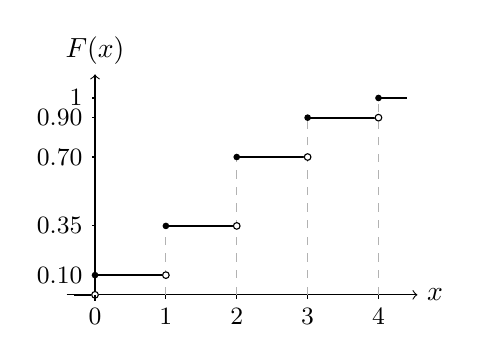
\begin{tikzpicture}[x=0.9cm,y=2.5cm]
  \draw[->] (-0.4,0) -- (4.55,0) node[right] {$x$};
  \draw[->] (0,-0.03) -- (0,1.12) node[above] {$F(x)$};

  \draw[dashed,gray!60] (1,0) -- (1,0.35);
  \draw[dashed,gray!60] (2,0) -- (2,0.70);
  \draw[dashed,gray!60] (3,0) -- (3,0.90);
  \draw[dashed,gray!60] (4,0) -- (4,1.00);

  \draw[thick] (-0.3,0) -- (0,0);
  \draw[thick] (0,0.10) -- (1,0.10);
  \draw[thick] (1,0.35) -- (2,0.35);
  \draw[thick] (2,0.70) -- (3,0.70);
  \draw[thick] (3,0.90) -- (4,0.90);
  \draw[thick] (4,1.00) -- (4.4,1.00);

  \filldraw[white] (0,0) circle (1.2pt);
  \draw (0,0) circle (1.2pt);
  \fill (0,0.10) circle (1.2pt);
  \filldraw[white] (1,0.10) circle (1.2pt);
  \draw (1,0.10) circle (1.2pt);
  \fill (1,0.35) circle (1.2pt);
  \filldraw[white] (2,0.35) circle (1.2pt);
  \draw (2,0.35) circle (1.2pt);
  \fill (2,0.70) circle (1.2pt);
  \filldraw[white] (3,0.70) circle (1.2pt);
  \draw (3,0.70) circle (1.2pt);
  \fill (3,0.90) circle (1.2pt);
  \filldraw[white] (4,0.90) circle (1.2pt);
  \draw (4,0.90) circle (1.2pt);
  \fill (4,1.00) circle (1.2pt);

  \foreach \x in {0,1,2,3,4}
    \draw (\x,0) -- (\x,-0.02) node[below] {\small \x};
  \foreach \y/\label in {0.10/0.10,0.35/0.35,0.70/0.70,0.90/0.90,1.00/1}
    \draw (0,\y) -- (-0.04,\y) node[left] {\small \label};
\end{tikzpicture}
\end{tabular}
\end{center}

\textbf{(b1)} \[
P(1<X\le 3)=P(X=2)+P(X=3)=0.35+0.20=0.55.
\]

\textbf{(b2)} \[
P(1<X\le 3)=F(3)-F(1)=0.90-0.35=0.55.
\]
\endgroup
\end{solution}

\vfill

% -------------------------------------------------------
\newpage
\AddToShipoutPictureFG*{\DrawQuestionPageTemplate}
\vspace*{\QuestionTopOffset}

\question
\begingroup
\small
\noindent Industrial control devices produced on an assembly line are tested at a quality control station at the end of the day. The quality engineer denotes the number of critical nonconformities detected during a shift by the random variable \(X\). The aim is to analyze the average error load of the process and its variability.

According to the test records, the probability distribution of \(X\) is as follows:
\[
\begin{array}{c|cccccc}
x & 0 & 1 & 2 & 3 & 4 & 5\\
\hline
P(X=x) & 0.08 & 0.17 & 0.25 & 0.22 & 0.18 & 0.10
\end{array}
\]

Accordingly:
\begin{enumerate}[nosep]
    \item[\textbf{(a)}] Find the expected value, i.e., \(E(X)\).
    \item[\textbf{(b)}] Find the value of \(E(X^2)\).
    \item[\textbf{(c)}] Find the variance, i.e., \(\mathrm{Var}(X)\).
\end{enumerate}
\endgroup

\begin{solution}
\begingroup
\small
\textbf{(a)} \[
E(X)=\sum xP(X=x)=0(0.08)+1(0.17)+2(0.25)+3(0.22)+4(0.18)+5(0.10)=2.55.
\]

\textbf{(b)} \[
E(X^2)=\sum x^2P(X=x)=1^2(0.17)+2^2(0.25)+3^2(0.22)+4^2(0.18)+5^2(0.10)=8.53.
\]

\textbf{(c)} \[
\mathrm{Var}(X)=E(X^2)-[E(X)]^2=8.53-(2.55)^2=8.53-6.5025=2.0275.
\]
\endgroup
\end{solution}

\vfill

% -------------------------------------------------------
\newpage
\AddToShipoutPictureFG*{\DrawQuestionPageTemplate}
\vspace*{\QuestionTopOffset}

\question
\begingroup
\small
\noindent The probability density function of the continuous random variable \(X\) is defined as follows:

\[
f(x)=
\begin{cases}
c\,x, & 0\le x\le 1,\\[4pt]
c(2-x), & 1< x\le 2,\\[4pt]
0, & \text{otherwise}.
\end{cases}
\]

Accordingly:
\begin{enumerate}[nosep]
    \item[\textbf{(a)}] Find the value of \(c\) so that \(f(x)\) can be a probability density function.
    \item[\textbf{(b)}] Find the probability \(P(0.5\le X\le 1.5)\).
    \item[\textbf{(c)}] Find the value of \(E(X)\).
    \item[\textbf{(d)}] Find the variance \(\mathrm{Var}(X)\).
\end{enumerate}
\endgroup

\begin{solution}
\begingroup
\small
\textbf{(a)} \[
\int_0^1 cx\,dx+\int_1^2 c(2-x)\,dx=\frac{c}{2}+\frac{c}{2}=c=1.
\]
Therefore \(\boxed{c=1}\).

\textbf{(b)} \[
P(0.5\le X\le 1.5)=\int_{0.5}^{1}x\,dx+\int_{1}^{1.5}(2-x)\,dx
=\frac{3}{8}+\frac{3}{8}=\frac{3}{4}=0.75.
\]

\textbf{(c)} \[
E(X)=\int_0^1 x(x)\,dx+\int_1^2 x(2-x)\,dx
=\int_0^1 x^2\,dx+\int_1^2 (2x-x^2)\,dx=1.
\]

\textbf{(d)} \[
E(X^2)=\int_0^1 x^2(x)\,dx+\int_1^2 x^2(2-x)\,dx
=\int_0^1 x^3\,dx+\int_1^2 (2x^2-x^3)\,dx=\frac{7}{6}.
\]
\[
\mathrm{Var}(X)=E(X^2)-[E(X)]^2=\frac{7}{6}-1=\frac{1}{6}.
\]
\endgroup
\end{solution}

\vfill

\end{questions}

\end{document}